\chapter{Verificaci\'{o}n y evaluaci\'{o}n}
En este cap\'itulo se detallar\'an las pruebas
que se han llevado a cabo para verificar que el software
cumple todos los requisitos correctamente.

Las pruebas representan los comportamientos que debe
tener la aplicaci\'on, es decir, lo que se prueban son los
casos de uso y subcasos de uso, no si cada m\'etodo
realiza de forma correcta su tarea.

\section{Cargar XML}

\subsection{Preparaci\'on de las pruebas}
Para poder probar este comportamiento no se requiere de ninguna preparaci\'on 
especial.

\subsection{Pruebas realizadas}
\subsubsection{Cargar XML nada m\'as abrir la aplicaci\'on}
Se prueba el comportamiento que debe tener la aplicaci\'on al cargar
un XML para empezar a trabajar, lo que se conoce como un arranque en fr\'io.

\paragraph{Resultado esperado}
Todos los datos cargados en la aplicaci\'on eliminados, 
tanto intervalos creados, como visualizadores de datos,
contenedores... todo debe haberse borrado de memoria volviendo a un estado inicial
de la aplicaci\'on.

\paragraph{Resultado obtenido}
Todos los datos se han borrado excepto los elementos del \'arbol de observaciones
y propiedades. 

\paragraph{Acciones realizadas}
Modificado el m\'etodo de cargar XML para limpiar tambi\'en los elementos del
\'arbol.

\subsubsection{Cargar XML cuando ya haya un XML cargado}
Esta prueba contempla dos situaciones, 
ya que este comportamiento se da cuando hay
hay un XML cargado pero no se ha hecho nada, como cuando hay un XML cargado justo
despu\'es de guardar un paso o situaci\'on a disco.

\paragraph{Resultado esperado}
Todos los datos cargados en la aplicaci\'on eliminados, 
tanto intervalos creados, como visualizadores de datos,
contenedores... todo debe haberse borrado de memoria volviendo a un estado inicial
de la aplicaci\'on.

\paragraph{Resultado obtenido}
Todos los datos se han borrado excepto los elementos del \'arbol de observaciones
y propiedades. 

\paragraph{Acciones realizadas}
Modificado el m\'etodo de cargar XML para limpiar tambi\'en los elementos del
\'arbol.

\subsubsection{Cargar XML habiendo un XML cargado y con uno o varios intervalos guardados}
Esta prueba contempla el hecho de cargar un XML cuando ya hemos creado uno o varios
intervalos listos para ser guardados

\paragraph{Resultado esperado}
Todos los datos cargados en la aplicaci\'on eliminados, sobre todo dando mucha importancia a
que se eliminen los intervalos.

\paragraph{Resultado obtenido}
Todos los datos se han eliminado correctamente.

\paragraph{Acciones realizadas}
Ninguna por obtener el resultado esperado.

\section{Crear intervalo}
\subsection{Preparaci\'on de las pruebas}
Para poder crear un intervalo es necesario tener cargado un XML, y adem\'as haber cargado,
al menos, una propiedad en el sistema y tener un rango seleccionado.

\subsection{Pruebas realizadas}
\subsubsection{Guardar el rango no habiendo ninguno guardado previamente}
Se probar\'a si guarda correctamente un rango cu\'ando no hay ninguno guardado de antes.
Aqu\'i se pone a prueba el comportamiento de cuando se van a guardar rangos que no entran
en conflicto con ninguno.

\paragraph{Resultado esperado}
El rango se guarda en la colecci\'on de intervalos a guardar en disco, y se 
muestra un mensaje informando de que se ha a\~nadido correctamente.

\paragraph{Resultado obtenido}
El resultado obtenido es el esperado, se ha a\~nadido correctamente y se muestra
el mensaje de informaci\'on

\paragraph{Acciones realizadas}
Ninguna al obtener el resultado esperado

\subsubsection{Guardar un rango que solape a otro previamente guardado}
Esta prueba contiene a su vez cuatro pruebas que han sido agrupadas, ya que un intervalo
se puede superponer a otro de cuatro maneras, tal y como se ve en la Figura \ref{fig:ModosSolapamiento}.

\begin{figure}[H]
\centering
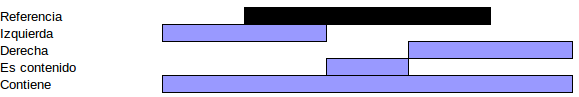
\includegraphics[width=0.9\linewidth]{./Figures/ModosSolapamiento.png}
\caption{Modos solapamiento}
\label{fig:ModosSolapamiento}
\end{figure}

El cuadrado negro representa el intervalo que est\'a guardado en el sistema, y azules-lilas
representan el que va a intentarse guardar.

\paragraph{Resultado esperado}
Las cuatro veces que intenten guardarse esos intervalos debe salir un mensaje informando
de que el intervalo a guardar solapa con alguno previamente guardado, y no debe
guardarse.

\paragraph{Resultado obtenido}
Para esos cuatro casos se obtiene el resultado esperado, pero en el caso extremo
en el que el intervalo guardado y el intervalo a guardar son iguales se guarda, dando
lugar a incongruencias. Hay que tener en cuenta que en el caso de empezar y acabar
en el mismo punto es la situaci\'on de ``contiene".

\paragraph{Acciones realizadas}
Se ajustan las comprobaciones, cambio los ``<" \ y ``>" por ``<=" \ y ``=>".

\subsubsection{Guardar un intervalo vac\'io}
Lo que se prueba aqu\'i es que no se pueda guardar un intervalo vac\'io, ya que ser\'ia
llenar el XML resultante con etiquetas vac\'ias. Para probar se seleccionar\'a un rango
vac\'io y se pinchar\'a en crear intervalo.

\paragraph{Resultado esperado}
Un mensaje de advertencia indicando que es necesario seleccionar un rango, y
el intervalo no se guardar\'a.

\paragraph{Resultado obtenido}
No se muestra nada y se guarda el intervalo

\paragraph{Acciones realizadas}
Se crea la condici\'on en la que se muestre el
di\'alogo y que no se guarde nada, si el inicio del intervalo
es igual al final del intervalo.

\section{Guardar paso o situaci\'on}
\subsection{Preparaci\'on de las pruebas}
Para guardar un paso o situaci\'on, no se necesita ninguna preparaci\'on especial.
Para guardar un paso o una situaci\'on que tenga sentido, y datos se requiere haber creado al menos un 
intervalo. 

\subsection{Pruebas realizadas}
\subsubsection{Guardar paso}
Al pinchar en guardar paso, se mostrar\'a el di\'alogo de guardado.

\paragraph{Resultado esperado}
Si el usuario decide guardar, se guardar\'an todos los intervalos
creados previamente y se descargar\'an de memoria. Si no se decide
guardar, no se har\'a nada y se podr\'a seguir trabajando.

\paragraph{Resultado obtenido}
Los resultados son los esperados.

\paragraph{Acciones realizadas}
Ninguna.

\section{A\~nadir v\'ideo}
\subsection{Preparaci\'on de las pruebas}
Para a\~nadir un v\'ideo no se requiere de acciones previas.
Se pueden a\~nadir en cualquier momento.

\subsection{Pruebas realizadas}
\subsubsection{A\~nadir un v\'ideo que no existe}

\subsubsection{A\~nadir un v\'ideo que ya existe}

\section{Cargar propiedad u observaci\'on}

\section{Cerrar observaci\'on}

\section{Cerrar propiedad}

\section{Seleccionar rango}